\section{Teorema de Cauchy}

El teorema de Cauchy (o integral de Cauchy) es considerado el teorema fundamental de la integración compleja. El enunciado del teorema usa implícitamente el teorema de la curva de Jordan, que establece que una curva continua, simple y cerrada en el plano separa al plano en dos conjuntos abiertos. Uno de estos conjuntos es no acotado y se llama el \textit{exterior}, y el otro es acotado y se llama el \textit{interior}. La curva misma no pertenece a ninguno de estos conjuntos, pero marca la frontera de ambos.

\begin{figure}[ht]
  \centering
  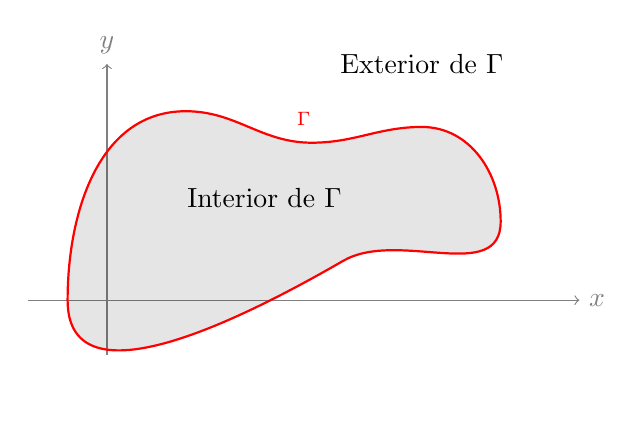
\begin{tikzpicture}
    \draw[->,gray] (-1,0) -- (6,0) node[right] {$x$};
    \draw[->,gray] (0,-0.7) -- (0,3) node[above] {$y$};

    \draw[thick,red,fill=black,fill opacity=0.1] (-0.5,0) to [out=90,in=180] (1,2.4)
    to [out=0,in=180] (2.6,2) 
    to [out=0,in=180] (4,2.2)
    to [out=0,in=90] (5,1)
    to [out=-90,in=30] (3,0.5)
    to [out=210,in=-90] (-0.5,0);
    \node[red] at (2.5,2.3) {\scriptsize$\Gamma$};

    \node at (2,1.3) {Interior de $\Gamma$};
    \node at (4,3) {Exterior de $\Gamma$};
  \end{tikzpicture}
  \caption{Teorema de la curva de Jordan.}
\end{figure}

A pesar de que esta conclusión puede parecer obvia para las curvas cerradas que se suelen dibujar, es difícil de probar debido a la generalidad de su enunciado. 

En la sección \ref{sec:1_curvas_y_regiones_en_el_plano_complejo} estuvimos analizando algunas regiones del plano complejo y sus propiedades. Esto lo hicimos para poder definir el dominio de una función compleja. Ahora vamos a profundizar algunos aspectos sobre las regiones del plano complejo para poder enunciar correctamente el teorema de Cauchy.

\begin{definition}[Trayectoria]
  Una trayectoria es una curva simple, suave a trozos. Una trayectoria pertenece a un conjunto $S$ si su gráfica está contenida dentro de $S$
\end{definition}

Algunas de las curvas paramétricas que hemos realizado anteriormente (como la figura \ref{fig:ejemplo_parabola_gamma}) son trayectorias en $\mathbb{C}$. Así, una trayectoria es una concatenación de curvas suaves que no se cruzan a sí mismas.

\begin{definition}[Conjunto conexo]
  Un conjunto $S$ de números complejos es conexo si, dados dos puntos cualesquiera de $z$ y $w$ en $S$, existe una trayectoria en $S$ que tiene a $z$ y a $w$ como puntos extremos.
\end{definition}

$S$ es conexo si es posible ir desde cualquier punto de $S$ a cualquier otro punto moviéndose a lo largo de alguna trayectoria totalmente contenida en $S$. Un disco abierto es conexo, así como también lo es un disco cerrado (ver sección \ref{sec:1_curvas_y_regiones_en_el_plano_complejo}).

\begin{definition}[Trayectoria simple cerrada]
  Es una trayectoria cerrada (el punto inicial $\Gamma(a)$ es igual al punto final $\Gamma(b)$) sin autointersecciones y que no se toca así misma. Por ejemplo una circunferencia como $\Gamma(t)=e^{jt}$ con $t\in[0,2\pi]$ es simple, ya que el único punto de intersección es el de inicio y fin (que indican que es cerrada). Si el intervalo de $\Gamma$ fuese $t\in[0,4\pi]$, la trayectoria \textbf{no es simple}, ya que un giro lo hace sobre el anterior. Descartado que trayectorias como un ``ocho'' como se muestra en la figura \ref{fig:trayectoria_nosimple} no son simples.
\end{definition}

\begin{figure}[ht]
  \centering
  \begin{subfigure}[b]{0.4\textwidth}
    \centering
    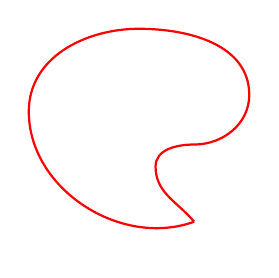
\begin{tikzpicture}[scale=0.7]
      \draw[red,thick] (1,0) to [out=200,in=270] (-2,2)
      to [out=90,in=180] (0,3.5)
      to [out=0,in=90] (2,2.3)
      to [out=270,in=0] (1,1.4)
      to [out=180,in=90] (0.3,1)
      to [out=270,in=130] (1,0);
    \end{tikzpicture}
    \caption{Simple}
  \end{subfigure}
  \hspace{1cm}
  \begin{subfigure}[b]{0.4\textwidth}
    \centering
    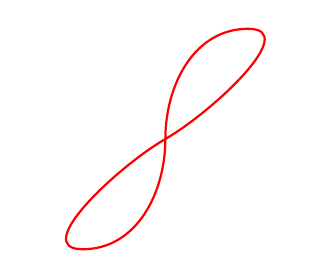
\begin{tikzpicture}[scale=0.7]
      \draw[red,thick] (0,0) to [out=90,in=180] (1.5,2)
      to [out=0,in=30] (0,0) 
      to [out=210,in=180] (-1.5,-2)
      to [out=0,in=270] (0,0);
    \end{tikzpicture}
    \caption{No simple}
    \label{fig:trayectoria_nosimple}
  \end{subfigure}
  \caption{Trayectorias cerradas}
\end{figure}


Una trayectoria simple y cerrada cumple con el teorema de Jordan. Es decir, separa claramente el plano en dos conjuntos: el interior y el exterior.

\begin{definition}[Simplemente conexo]
  Un conjunto $S$ de números complejos es simplemente conexo si toda trayectoria cerrada en $S$ encierra únicamente puntos de $S$.
  \label{def:simplemente_conexo}
\end{definition}

Todo disco abierto es simplemente conexo. Si dibuja una trayectoria cerrada en un disco abierto, esta trayectoria cerrada encerará solamente puntos en el disco abierto. El anillo o corona de la figura \ref{fig:corona_complx} no es simplemente conexo. A pesar de ser conexo, se puede dibujar una trayectoria cerrada contenida en el anillo que encierra puntos que no pertenecen al anillo (son aquellos puntos excluidos por la frontera interna).

\begin{definition}[Dominio simplemente conexo]
  Como se vió en la sección \ref{sec:1_curvas_y_regiones_en_el_plano_complejo} un dominio es un conjunto conexo abierto. Ahora, decimos que un dominio $D$ es simplemente conexo si además de cumplir con la definición de dominio cumple con la definición \ref{def:simplemente_conexo}.
\end{definition}

Por ejemplo, en la figura \ref{fig:doblemente_conexo} si se traza una trayectoria circular $\Gamma$ dento de la región pintada, esta encierra puntos que no pertenecen a $D$ (que son los puntos dentro de la elipse pequeña que delimita el interior de la región). Lo mismo sucede con la región de la figura \ref{fig:triplemente_conexo}.

Por otro lado, si se observan las figuras \ref{fig:simple_simple} y \ref{fig:simple_complicada} es imposible trazar una curva $\Gamma$ dentro de la región pintada que encierre puntos fuera de la región.

\begin{figure}[ht]
  \centering
  \begin{subfigure}[b]{0.24\textwidth}
    \centering
    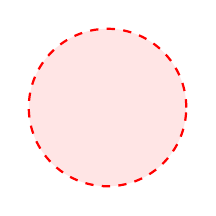
\begin{tikzpicture}
      \draw[thick,red,dashed,fill=red!10] (0,0) circle (1);
    \end{tikzpicture}
    \caption{Simple}
    \label{fig:simple_simple}
  \end{subfigure}
  \hfill
  \begin{subfigure}[b]{0.24\textwidth}
    \centering
    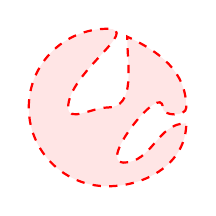
\begin{tikzpicture}
      \draw[thick,red,dashed,fill=red!10] (-1,0) to [out=90,in=180] (0,1)
      to [out=0,in=90] (-0.5,0)
      to [out=270,in=180](0,0)
      to [out=0,in=270] (0.25,0.9)
      to [out=335,in=90] (1,0)
      to [out=270,in=270] (0.7,0)
      to [out=90,in=180] (0.2,-0.7)
      to [out=0,in=180] (1,-0.2)
      to [out=270,in=0] (0,-1)
      to [out=180,in=270] (-1,0);
    \end{tikzpicture}
    \caption{Simple}
    \label{fig:simple_complicada}
  \end{subfigure}
  \hfill
  \begin{subfigure}[b]{0.24\textwidth}
    \centering
    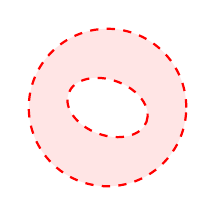
\begin{tikzpicture}
      \draw[thick,red,dashed,fill=red!10] (0,0) circle (1);
      \draw[thick,red,dashed,rotate=-20,fill=white] (0,0) ellipse [x radius=15pt,y radius=10pt];
    \end{tikzpicture}
    \caption{Doble}
    \label{fig:doblemente_conexo}
  \end{subfigure}
  \hfill 
  \begin{subfigure}[b]{0.24\textwidth}
    \centering
    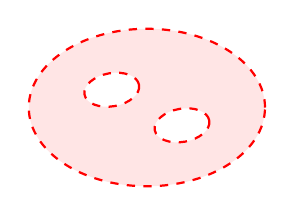
\begin{tikzpicture}
      \draw[thick,red,dashed,fill=red!10] (0,0) ellipse [x radius=1.5, y radius=1];
      \draw[thick,red,dashed,rotate=10,fill=white] (-0.4,0.3) ellipse [x radius=10pt,y radius=6pt];
      \draw[thick,red,dashed,rotate=10,fill=white] (0.4,-0.3) ellipse [x radius=10pt,y radius=6pt];
    \end{tikzpicture}
    \caption{Triple}
    \label{fig:triplemente_conexo}
  \end{subfigure}
  \caption{Conexidad de dominios}
\end{figure}


Ahora si, estamos listos para enunciar el teorema de Cauchy.

\subsection[Enunciado del teorema]{El teorema de Cauchy}

\begin{theorem}[Teorema de Cauchy]
  Sea $f(z)$ analítica en un dominio simplemente conexo $D$, entonces para toda trayectoria simple cerrada $\Gamma$ en $D$ se cumple que
  \[
    \oint_\Gamma f(z)dz=0
  \]
\end{theorem}

Con este teorema, solo se cumple si la función es analítica. Si $f(z)$ no es analítica nada podemos asegurar con respecto a su resultado, ya que puede o no ser cero. Veamos un ejemplo de cada una.

\begin{example}
  Dada $f(z)=e^z$ calcular su integral sobre la curva $\Gamma(t)=e^{jt}$ con $t\in[0,2\pi]$ que es la cirfunferencia unitaria. Como $f$ es analítica para todo $z\in\mathbb{C}$, entonces
  $$
  \oint_\Gamma e^{z}dz = 0
  $$
  ya que $f$ cumple con el teorema de Cauchy.
  \label{ej:teorema_de_cauchy_no_analitica}
\end{example}

\begin{example}
  Dada $f(z)=\frac{1}{z^2}$, calcular la integral sobre la misma curva $\Gamma$ del ejemplo \ref{ej:teorema_de_cauchy_no_analitica}. 

  Como $f$ no es analítica en $z=0$ entonces no podemos aplicar el teorema de Cauchy. La resolvemos como una integral de línea usual.
  $$
  z'(t)=je^{jt} \qquad f(z(t))=\frac{1}{e^{j2t}}
  $$
  Entonces:
  \begin{gather*}
    \oint_\Gamma f(z)dz = \int_0^{2\pi} j\frac{e^{jt}}{(e^{jt})^2}dt = j\int_0^{2\pi} e^{-jt}dt = \left[ j\frac{e^{-jt}}{-j} \right\lvert _0^{2\pi} \\ 
    \oint_\Gamma f(z)dz = -e^{-j2\pi}+e^{0} = -1+1=\boxed{0}
  \end{gather*}
  Por tanto, la condición de que $f$ sea analítica en $D$ es suficiente para cumplir el teorema de Cauchy. Es decir, este ejemplo ha servido para demostrar que existen funciones no analíticas que al integrarlas sobre una curva cerrada simple, dan como resultado cero.
\end{example}

\subsection{Demostración del teorema de Cauchy}

Habiamos visto en la sección \ref{sec2:integral_cmplx_en_terminos_reales} que una integral compleja puede ser expresada en término de integrales reales como sigue
\begin{equation}
\oint_\Gamma f(z)dz = \oint_\Gamma u\,dx - v\,dy + j\oint_\Gamma v\,dx + u\,dy 
\label{eq:premisa_demostracion_cauchy}
\end{equation}
Debido a que suponemos que $f$ es una función que cumple con el teorema de Cauchy, entonces $f$ es analítica en $D$, y por tanto $f'(z)$ existe en $D$. Esto implica que $f$ también cumple con las ecuaciones de \textit{Cauchy-Riemann}. Entonces, la ecuación \ref{eq:premisa_demostracion_cauchy} podemos escribirla usando el teorema de Green (ver sección \ref{chpt:recordatorios}) como sigue
\begin{align}
  \label{eq:teorema_de_green_aplicado_a_cauchy_1}
  \oint_\Gamma u\,dx - v\,dy &= \iint_R v_x - u_y \,dA \\ 
  \label{eq:teorema_de_green_aplicado_a_cauchy_2}
  \oint_\Gamma v\,dx + u\,dy &= \iint_R -u_x - v_y \,dA
\end{align}
Como hemos dicho que $f$ es analítica y $u(x,y)$ y $v(x,y)$ cumplen las ecuaciones de CR. Si observamos el integrando del miembro derecho de las ecuaciones \eqref{eq:teorema_de_green_aplicado_a_cauchy_1} y \eqref{eq:teorema_de_green_aplicado_a_cauchy_2} no son más que las ecuaciones de CR reordenadas:
$$
v_y-u_x=0 \rightarrow u_x = v_y  \qquad -u_x-v_y = 0 \rightarrow v_y = -u_x
$$
de tal manera, que no queda más alternativa que 
$$
\oint_\Gamma f(z)dz = \oint_\Gamma u\,dx - v\,dy + j\oint_\Gamma v\,dx + u\,dy = 0
$$
